\section{Recursion (Divide \& Conquer)}
\begin{itemize}
\item Recursion is like Induction's twin brother, whereas induction is similar to movie filmed, and recursion is similar to movie backward.
\item Recursion design may be most important course topic.
\item Recursion is a type of reduction. \footnote{Reduction is to solve problem A using a black box for B. Typically B is smaller.}
\end{itemize}

\subsection{Definition of Recursion: a Powerful type of reduction}
\begin{enumerate}
\item if problem size very small (think $\mathcal{O}(1)$), just solve it.
\item reduce to one or more small instances of some problem.
\end{enumerate}

\question How are the smaller (but not $\mathcal{O}(1)$ size) problem solved?

Not your problem! Handled by the recursion fairy.

\subsection{Tower of Hanoi}
\subsubsection{Description of Problem}
\begin{itemize}
    \item 3 pegs, which hold n distinct sized disks.
    \item initially $tmp$, $dst$ empty and $src$ has all disks sorted.
    \item 3 rules:
    \begin{enumerate}
        \item larger cannot be placed on smaller.
        \item only one disks can move at a time.
        \item move all disks to $dst$.
    \end{enumerate}
\end{itemize}

\question How long until the world end?

\subsubsection{Analysis}
A small hint: not consider the smallest first, but the largest first.

In order to move the largest disk:
\begin{itemize}
    \item $dst$ has to be empty.
    \item $src$ has only largest one.
    \item $tmp$ has $n-1$ disks sorted.
\end{itemize}

So we must:
\begin{enumerate}
    \item move $n-1$ disks from $src$ to $tmp$\tikzmark{hanoi1}{.}
    \item move largest from $src$ to $dst$\tikzmark{hanoi2}{.}
    \item move $n-1$ disk from $tmp$ to $dst$\tikzmark{hanoi3}{.}

    \begin{tikzpicture}[remember picture,overlay,node distance = 3cm]
        \node (hanoi12descr) [right =of hanoi2]{Don't know how to do.};
        \node (hanoi12descrdescr) [below =1cm of hanoi12descr]{\textbf{Don't think about it!!}};
        \draw[red,->,thick] (hanoi1) to [in=-180,out=0] (hanoi12descr);
        \draw[blue,->,thick] (hanoi3) to [in=-180,out=0] (hanoi12descr);
        \draw[purple,->,thick] (hanoi12descr) to [in=90,out=-90] (hanoi12descrdescr);
    \end{tikzpicture}
\end{enumerate}

Don't think about how to move $n-1$ disks, recursion fairy will do it.

\begin{algorithm}[h]
    \caption{Recursive Hanoi}\label{rec_hanoi}
    \begin{algorithmic}
        \Procedure{Hanoi}{$n, src, dst, tmp$}
            \If{$n>0$}
                \State \ProcedureName{Hanoi}{n-1, src, tmp, dst}
                \State Move disk $n$ from $src$ to $dst$.
                \State \ProcedureName{Hanoi}{n-1, tmp, dst, src}
            \EndIf
        \EndProcedure
    \end{algorithmic}
\end{algorithm}

How many moves in \cref{rec_hanoi} ?

Let $T(n)$ be the total moves for $n$ disks.
\begin{align*}
    T(0) &= 0 \\
    T(1) &= 1 \\
    T(n) &= T(n-1) + 1 + T(n-1) \\
         &= 2T(n-1) + 1
\end{align*}

``Solve'' the recurrence.
\[\sum_{l=1}^n 2^{l-1} = 2^n - 1\]

\subsection{Binary Search}

\AlgoInput Given a value $val$, and sorted aray $A[1 \ldots n]$.

\AlgoOutput Is $val$ contained in $A$?

\begin{algorithm}[H]
\caption{Binary Search Algorithm}\label{bianry_search}
\begin{algorithmic}[1]
\Procedure{Bin}{$val, low, high$}
  \If{$high < low$}
    \Return Not Found
  \EndIf
  \State $mid = \big\lfloor\frac{high + low}{2}\big\rfloor$
  \If{$val < A[mid]$}
    \Return \ProcedureName{Bin}{val, low, mid-1}
  \EndIf
  \If{$val > A[mid]$}
    \Return \ProcedureName{Bin}{val,mid+1,high}
  \EndIf
  \Return $mid$
\EndProcedure
\end{algorithmic}
\end{algorithm}

To find whether $val$ is contained in $A[1\ldots n]$, call \ProcedureName{Bin}{val,1,n}.

Let $m = high - low + 1$,

\begin{align}
T(m) & \leq \max\bigg\{T\Big(\Big\lfloor\frac{m-1}{2}\Big\rfloor\Big)\tikzmark{floorceil},
                       T\Big(\Big\lceil\frac{m-1}{2}\Big\rceil\Big)\bigg\}
                       + \Theta(1)\\
     & \leq T\big(\frac{m}{2}\big) + \Theta(1) \\
T(m) & = T\big(\frac{m}{2}\big) + 1 \\
T(m) & = \Theta(1) \text{ for } m = \Theta(1) \tikzmark{notesont}{ }
    \begin{tikzpicture}[remember picture,overlay,node distance = 2cm]
        \node (floorceildescr) [below right =of floorceil, text width=5cm]{\footnotesize{Floor and Ceilings has differences in constant time.}};
        \node (notesontdescr) [below right=1cm and 2cm of notesont, text width=6cm]{\footnotesize{A constant size problem should has a constant solution.}};
        \draw[red,->,thick] (floorceil) to [in=-180,out=-90] (floorceildescr);
        \draw[red,->,thick] (notesont) to [in=-180,out=0] (notesontdescr);
    \end{tikzpicture}
\end{align}

To think the running time in another way:

\begin{align*}
T(m) &= T\Big(\frac{m}{2}\Big) + 1 \\
     &= T\Big(\frac{m}{2\times 2}\Big) + 1 + 1 \\
     &= T\Big(\frac{m}{2\times 2\times 2}\Big) + 1 + 1 + 1
\end{align*}

Counting the number of times divide by 2 to get to 1, i.e.

\[\frac{m}{2^x} = 1 \rightarrow m = 2^x \rightarrow x = \lg{m}\]


\subsection{Maximum Sub-array Sum}

\subsubsection{Description of Problem}

\AlgoInput Given an unsorted array $A[1 \ldots n]$ of integers,
including both negative and positive number.

\AlgoOutput $\displaystyle\max_{i\leq j}\bigg\{\sum_{k=i}^j{A[k]}, 0\bigg\}$.

\subsubsection{Analysis}

\textbf{The Naive Solution}

Let $W[i][j] = \displaystyle\sum_{k=i}^j{A[k]}$ for $i \leq j$.
Return $\max\{0, \max\{W[i][j]\}\}$.
The running time of this brute force solution is$T(n) = \displaystyle\sum_{j=1}^n{\sum_{i=1}^j{(j-i+1)}} = \Theta(n^3)$

\noindent\textbf{Think Recursively!}

Let $maxSum(i,j)$ be the maximum sub-array sum in $A[1 \ldots n]$ or $0$.
The solution is $maxSum(1,n)$.\tikzmark{notesonmaxsum}{ }
\begin{tikzpicture}[remember picture, overlay, node distance = 2cm]
    \node (notesonmaxsumdescr) [below right=0.3cm and 3cm of notesonmaxsum, text width=10cm]{\footnotesize{Can we express $maxSum(1,n)$ in term of $maxSum(1,n-1)$?}};
    \draw[red,->,thick] (notesonmaxsum) to [in=-180,out=0] (notesonmaxsumdescr);
\end{tikzpicture}

There are two cases:

\begin{itemize}
    \item $maxSum(1, n)$ does not include $A[n]$
        \[maxSum(1, n) = maxSum(1, n-1)\]
    \item $maxSum(1, n)$ does include $A[n]$
        \[maxSum(1, n) = maxEndAt(1, n)\]
\end{itemize}

$maxEndAt(i, j)$ is the maximum sub-array sum in $A[i, j]$ restricted to include $A[j]$.

Here comes the recursive version algorithm to solve this problem, showing in .

\begin{algorithm}[H]
\caption{Recursive Solution for Maximum Sub-Array Sum Problem}\label{recur_max_sub_sum}
\begin{algorithmic}[1]
\Procedure{maxSum}{$i, j$}
  \If{$j < i$}
    \Return $0$
  \EndIf
  \State $x = $\ProcedureName{maxEndAt}{i, j}
  \Return $\max\{x, \ProcedureName{maxSum}{i, j-1}\}$
\EndProcedure
\Procedure{maxEndAt}{$i, j$}
    \If{$j < i$}
        \Return $0$
    \EndIf
    \Return $\max\{A[n], A[n] + \ProcedureName{maxEndAt}{i, j-1}\}$
\EndProcedure
\end{algorithmic}
\end{algorithm}

The running time for \ProcedureName{maxEndAt}{i, j} is $T(n) = T(n-1) + \Theta(1) = \Theta(n)$.
Accordingly, the running time for \ProcedureName{maxSum}{i, j} is
\begin{align*}
    T(m) &= T(m-1) + \Theta(m) \\
         &= T(m-1) + m \\
         &= \sum_{k=1}^m k \\
         &= \Theta(m^2) \\
\end{align*}

Can we do better?

Yes, use Divide and Conquer.

\subsubsection{Applying Divide \& Conquer on Max Sub-Array Sum Problem}

The key point of D\&C is try to get problem size down quickly.

\begin{algorithm}[H]
    \caption{Divide \& Conquer Solution for Maximum Sub-Array Sum Problem}\label{dc_max_sub_sum}
\begin{algorithmic}[1]
\Procedure{DCMaxSum}{$i, j$}
  \If{$j < i$}
    \Return $0$
  \EndIf
  \State $mid = \left\lfloor \frac{i + j}{2} \right\rfloor$
  \Return $\max\left\{
      \begin{array}{l}
          \ProcedureName{maxSum}{i, mid}, \\
          \ProcedureName{maxSum}{mid, j}, \\
          \ProcedureName{maxGoFrom}{i, mid} + \ProcedureName{maxGoFrom}{mid, j}
      \end{array}
  \right\}$
\EndProcedure
\end{algorithmic}
\end{algorithm}

If goes cross, must include $A[mid]$ and $A[mid+1]$.

The running time for \cref{dc_max_sub_sum} is
\[T(m) = 2T\big(\frac{m}{2}\big) + m\]
in which $m = j - i + 1$.


\begin{table}[!htb]
    \caption{Comparison Between Previous Two Method}

    \begin{minipage}{.65\linewidth}

        \centering
        \begin{tikzpicture}
        \Tree
        [.\node(root) {$n$};
                [.$\frac{n}{2}$
                    [.$\frac{n}{4}$ ]
                    [.$\frac{n}{4}$ ]
                ]
                [.\node(1level) {$\frac{n}{2}$};
                    [.$\frac{n}{4}$ ]
                    [.\node(2level) {$\frac{n}{4}$}; ]
                ]
            ]

            \node[right = 1cm of 2level] (2levelnote) {$n$};
            \node (1levelnote) at (1level -| 2levelnote) {$n$};
            \node (rootnote) at (root -| 2levelnote) {$n$};
            \path (2levelnote) -- (2level) node [midway] {$\Longrightarrow$};
            \path (1levelnote) -- (1level) node [midway] {$\Longrightarrow$};
            \path (rootnote) -- (root) node [midway] {$\Longrightarrow$};
        \end{tikzpicture}

        \justifying
        At each level, the running time sum is $n$.

        There are $\log n$ level in total.

        Thus, total running time is $\Theta(n\log n)$.

    \end{minipage}%
    \vline
    \begin{minipage}{.35\linewidth}
        \centering
        \begin{tikzpicture}
            \Tree
            [.\node(root) {$n$};
                [.\node(1level) {$n-1$};
                    [.\node(2level) {$n-2$}; ]
                ]
            ]

            \node[right = 1cm of 2level] (2levelnote) {$n$};
            \node (1levelnote) at (1level -| 2levelnote) {$n-1$};
            \node (rootnote) at (root -| 2levelnote) {$n-2$};
            \path (2levelnote) -- (2level) node [midway] {$\Longrightarrow$};
            \path (1levelnote) -- (1level) node [midway] {$\Longrightarrow$};
            \path (rootnote) -- (root) node [midway] {$\Longrightarrow$};
        \end{tikzpicture}

        \justifying
        \begin{align*}
            T(m) &= T(m-1) + \Theta(m) \\
                 &= \sum_{k=1}^m k \\
                 &= \Theta(m^2) \\
        \end{align*}
    \end{minipage}%
\end{table}

Can we do better?

The divide \& conquer solution constantly calculate the \ProcedureName{maxEndAt}{i, j}.
Memoizing the result leads to the dynamic programming solution as shown in next section.

\subsection{Solving Recurrence}
\subsubsection{Basic Idea}

Fail-safe method for any recurrence:
\begin{quote}
    Guess solution and prove correct with induction.
\end{quote}
The subtle point is: need to make the right guess!

\AlgoExample  Tower of Hanoi, $T(n) = 2T(n-1) + 1$, $T(1) = 1$.

\Claim $T(n) = 2^n -1$

\begin{proof}

    \BaseCase $T(1) = 2^1 -1 = 1$, true.

    \InductionStep Assume $T(m) = 2^m - 1$, for $m < n$.

    \[T(n) = 2T(n-1) + 1 = 2\times (2^{n-1} -1) + 1 = 2^n - 1\]

    Hold true for $n$.

    \InductionConclusion $T(n) = 2^n - 1$.
\end{proof}

\subsubsection{Typical Proving Method}
\AlgoExample maxSubArraySum, $T(n) = 2T(n/2) + \Theta(n)$.

\Claim $T(n) = \Theta(n \log n)$

\begin{proof}
    Still using induction, only show the induction phase below.

    Replace original statement with:
    \[T(n) = 2T(n/2) + n\]

    First, prove $T(n) \leq c \times n \log n$.
    \begin{align*}
        T(n) &= 2T\big(\frac{n}{2}\big) + n \\
             &\leq 2\times c \times \frac{n}{2} \times \log\big(\frac{n}{2}\big) + n \\
             &= c \times n \times \log(n-1) + n \\
             &= c \times n \times \log n + n(1-c) \\
             &= n\log n \text{ for } c = 1
    \end{align*}

    Then, prove $T(n) \geq c \times n \log n$. The same as previous one.
\end{proof}

\Note The constant in $T(n) = \bigO{n\log n}$ muse be specified.
And in $T(n) = c\times n\log n - bn$, sometimes $bn$ need to guess.

\subsubsection{Generalizing: Recursion Tree Method}
Generalize the equation $T(n) = T(n/2) + n$ to
\begin{equation}\label{main_recur_tree_eq}
    T(n) = a T\big(\frac{n}{b}\big) + f(n)
\end{equation}
where $a,b \geq 1$. The recursion tree for \cref{main_recur_tree_eq} is shown in \cref{main_recur_tree}.

\begin{figure}[H]
    \caption{Generalize Recursion Tree}\label{main_recur_tree}
\begin{tikzpicture}
    \Tree
    [.\node(root) {$f(n)$};
        [.$f\big(\frac{n}{b}\big)$
            [.\node[n] {$\ldots$};
                [.\node(ilevel) {$f\big(\frac{n}{b^i}\big)$}; ]
                \edge[n]; [.\node[n]{ }; ]
            ]
            [.\node[n] {$\ldots$}; ]
        ]
        [.\node(1level) {$f\big(\frac{n}{b}\big)$};
        ]
    ]

    \node[right = 2cm of 1level] (1levelnote) {$\displaystyle af\big(\frac{n}{b}\big)$};
    \node (ilevelnote) at (ilevel -| 1levelnote) {$\displaystyle a^if\big(\frac{n}{b^i}\big)$};
    \node (rootnote) at (root -| 1levelnote) {$f(n)$};
    \path (ilevelnote) -- (ilevel) node [very near start] {$\xRightarrow{\text{level sum}}$};
    \path (1levelnote) -- (1level) node [midway] {$\xRightarrow{\text{level sum}}$};
    \path (rootnote) -- (root) node [near start] {$\xRightarrow{\text{level sum}}$};
\end{tikzpicture}
\end{figure}

\observation

\begin{itemize}
    \item Level sum:  $\displaystyle a^i f\big(\frac{n}{b^i}\big)$
    \item Depth:      $\log_b n$
    \item Number of Leaves:    $a^{\log_b n}$
\end{itemize}

In total: $T(n) = \displaystyle \sum_{i=1}^{\log_b n} a^if\big(\frac{n}{b^i}\big)$, which often like a geometric series.

Look at the ratio of successive level sums:

\begin{equation}
    \cfrac{a^{i+1}f(\frac{n}{b^{i+1}})}{a^if(\frac{n}{b^i})}
    = a \times \frac{f(\frac{n}{b^{i+1}})}{f(\frac{n}{b^{i+1}})}
    =
    \begin{cases}
        > 1 \text{, then sum determined by the number of leaves.}\\
        < 1 \text{, then sum determined by root.} \\
        = 1 \text{, then sum determined by the depth or root.}\\
    \end{cases}
\end{equation}

A Special Case is that, $f(n) = n^c$, i.e. $f(n)$ is polynomial.
\begin{equation}\label{master_theorem}
    a \times \frac{f(\frac{n}{b^{i+1}})}{f(\frac{n}{b^{i+1}})}
    = a \times \frac{(\frac{n}{b^{i+1}})^c}{(\frac{n}{b^i})^c}
    = \frac{a}{b^c}
    =
    \begin{cases}
        > 1\text{, if } a>b^c\text{, then } T(n) = a^{\log_b n} = n^{\log_b a}\\
        < 1\text{, if } a<b^c\text{, then } T(n) = n^c\\
        = 1\text{, if } a=b^c\text{, then } T(n) = n^c\log_b n \\
    \end{cases}
\end{equation}

The \cref{master_theorem} is called the Master Theorem.

\subsubsection{Examples: \texorpdfstring{$T(n)=\sqrt{n}T(\sqrt{n})+n$}{T(n)=sqrt(n)T(sqrt(n))+n}}

The recursion tree are shown in \cref{fig:rt1}.
\begin{figure}[H]
    \caption{Recursion Tree for \texorpdfstring{$T(n)=\sqrt{n}T(\sqrt{n})+n$}{T(n)=sqrt(n)T(sqrt(n))+n}}\label{recur_tree_example1}
    \label{fig:rt1}
\begin{tikzpicture}
    \Tree
    [.\node(root) {$n$};
        \edge node [midway](notepoint) {  }; [.$n^{\frac{1}{2}}$
            [.\node(2level) {$n^{\frac{1}{4}}$}; ]
                \edge[n]; [.\node[n]{$\ldots$}; ]
        ]
        [.\node(1level) {$n^{\frac{1}{2}}$};
            \edge[n]; [.\node[n]{$\ldots$}; ]
            \edge[n]; [.\node[n]{  }; ]
        ]
    ]

    \node[above left= 2em and 2em of notepoint] (note) {There are $n^{\frac{1}{2}}$ sub-nodes.};
    \draw[red,->,thick] (notepoint) to [in=-45,out=-225] (note);
    \node[right = 2cm of 1level] (1levelnote) {$(n^{\frac{1}{2}})\times n^{\frac{1}{2}} = n$};
    \node (2levelnote) at (2level -| 1levelnote) {$\big[(n^{\frac{1}{2}})\times (n^{\frac{1}{4}})\big]\times (n^{\frac{1}{4}}) = n$};
    \node (rootnote) at (root -| 1levelnote) {$n$};
    \path (2levelnote) -- (2level) node [very near start] {$\xRightarrow{\text{level sum}}$};
    \path (1levelnote) -- (1level) node [midway] {$\xRightarrow{\text{level sum}}$};
    \path (rootnote) -- (root) node [near start] {$\xRightarrow{\text{level sum}}$};
\end{tikzpicture}
\end{figure}

\observation

Level sums: $\displaystyle \bigg(\prod_{i=1}^l n^{\frac{1}{2^i}}\bigg)\times \frac{1}{2^i} = n^{\displaystyle\bigg(\sum_{i=1}^l \frac{1}{2^i}\bigg) + \frac{1}{2^l}} = n^1$

Equal level sum, then what we need to know is the depth.
So the question turns to:

How many times apply $\sqrt{ n }$ (root function) until get to constant size?
\begin{align*}
    & n^{\frac{1}{2^i}} = c \\
    &\Rightarrow\frac{1}{2^i}\log n = \log c \\
    &\Rightarrow \log n = 2^i \log c \\
    &\Rightarrow \log\log n = i \log 2 + \log\log c \\
    &\Rightarrow i = \Theta(\log\log n) \\
\end{align*}

In total, the running time would be: $T(n) = \Theta(n\log\log n)$.


\subsubsection{Examples: \texorpdfstring{$T(n)=2T(\frac{n}{4}) + n\log n$}{T(n)=2T(n/4) + n log n}}
The recursion tree are shown in \cref{fig:rt2}.
\begin{figure}[H]
    \caption{Recursion Tree for \texorpdfstring{$T(n)=2T(\frac{n}{4}) + n\log n$}{T(n)=2T(n/4) + n log n}}
    \label{fig:rt2}
    \centering
\begin{tikzpicture}
    \Tree
        [.{$n \log n$} 
            [.{$\frac{n}{4} \log\frac{n}{4}$} ]
            [.{$\frac{n}{4} \log\frac{n}{4}$} ]
        ]
\end{tikzpicture}
\end{figure}

Level sum: $\displaystyle 2^i \frac{n}{4^i} \log\frac{n}{4^i} = \frac{n}{2^i}(\log (n-2i))$
is decreasing.

Thus, total running time is dominated by root, which is $T(n) = \Theta(n \log n)$.

To prove it, first prove the upper bound:
\begin{align*}
    T(n) &\leq 2c \times \frac{n}{4}\log\frac{n}{4} + n \log n \\
         &= \frac{1}{2}cn(\log n-2)+n \log n\\
         &= cn\log n \bigg(\frac{1}{2}+\frac{1}{c}\bigg) - cn \\
         &\leq cn\log n \text{ for } c = 2
\end{align*}
Then prove the lower bound, which is exactly the same steps as upper bound.


\subsubsection{Examples: \texorpdfstring{$T(n)=2T(\frac{n}{3}) + \sqrt{n}$}{T(n)=2T(n/3) + sqrt(n)}}
The recursion tree are shown in \cref{fig:rt3}.
\begin{figure}[H]
    \caption{Recursion Tree for \texorpdfstring{$T(n)=2T(\frac{n}{3}) + \sqrt{n}$}{T(n)=2T(n/3) + sqrt(n)}}
    \label{fig:rt3}
    \centering
\begin{tikzpicture}
    \Tree
        [.{$\sqrt{n}$} 
            [.{$\sqrt{\frac{n}{3}}$} ]
            [.{$\sqrt{\frac{n}{3}}$} ]
        ]
\end{tikzpicture}
\end{figure}

Level sum: $\displaystyle 2^i\sqrt{\frac{n}{3^i}} = \sqrt{n}\bigg(\frac{2}{\sqrt{3}}\bigg)$ is increasing.

Thus, total running time is dominated by number of leaves, which is
$2^{\log_3n}=n^{\log_32}$.

To prove it, first prove the lower bound:
\begin{align*}
    T(n) &\geq 2c\bigg(\frac{n}{3}\bigg)^{\log_32} + \sqrt{n} \\
         &= c \times n^{\log_32} + \sqrt{n} \\
         &\geq cn^{\log_32}
\end{align*}

Lower bound works for any $c$, but upper bound fails for any $c$.
In this case, we have to guess a upper bound:

Assume $T(n) \leq cn^{\log_32} - b\sqrt{n}$,
\[T(n) \leq 2 \times c \bigg(\frac{n}{3}\bigg)^{\log_32} - 2b\sqrt{\frac{n}{3}} + \sqrt{n}
= c \times n^{\log_32} + \sqrt{n}\bigg(1 - 2 \times \frac{b}{\sqrt{3}}\bigg)\]
for $\displaystyle \sqrt{n}\times\bigg(1 - \frac{2b}{\sqrt{3}}\bigg) = -b\sqrt{n}$.

